\chapter{Resultados}
\label{ch:resultados}
En este cap\'itulo se exponen resultados y an\'alisis de diferentes pruebas realizadas con la nueva versi\'on desarrollada del programa. La primera de las pruebas consiste en medir el desempe\~no de esta pipeline en t\'erminos de tiempo de ejecuci\'on y uso de memoria principal ocupada al procesar tres datasets (usados en el cap\'itulo \ref{ch:prev_work}) asociados a supernovas encontradas por HiTS\cite{hits}: SN14, SN18 y SN80. El segundo conjunto de experimentos corresponde al procesamiento sobre los 93 conjuntos de datos asociados a las supernovas encontradas por HiTS en el semestre de 2015. En ambos tipos de pruebas se busca compara el rendimiento y resultados del programa al emplear los diferentes filtros de Kalman implementados. Finalmente se muestran algunos resultados espec\'ificos obtenidos con el filtro unscented.
\bigskip


Para todas las experiencias se emple\'o umbrales de flujo y velocidad de flujo estimada de 200 [ADU] y 50 [ADU/d\'ia]. Adem\'as todas las im\'agenes procesadas poseen la misma dimensi\'on: $4094 \times 2046$ de alto por ancho, por lo que el campo \texttt{image\_size} de todos los filtros se configuraron en (4094, 2046). Por cada filtro se emplearon los siguientes valores de par\'ametros:

\subsection*{Filtro de Kalman B\'asico}
\begin{itemize}
\item \texttt{sigma\_a} : Se ocup\'o un valor de 0.1.
\item \texttt{init\_var} : La varianza inicial de flujo y velocidad de flujo se estableci\'o con un valor de 100.0.
\item Se determin\'o 0.0 como valor inicial para las estimaciones de flujo y velocidad de flujo (estado).
\end{itemize}
\subsection*{Filtro de Kalman de m\'axima correntrop\'ia}
\begin{itemize}
\item \texttt{sigma\_a}: Se defini\'o como 0.1
\item \texttt{sigma}: Valor de varianza usado por defecto en caso de no usar optimizaci\'on de Silverman.
\item \texttt{silverman}: \texttt{False}. Para estas pruebas no se us\'o el m\'etodo de Silverman para obtener distribuci\'on.
\item \texttt{std\_factor}: Se estableci\'o como 100.0. Al no usarse el m\'etodo de Silverman, tampoco se hace uso de este valor.
\item \texttt{epsilon}: Se asign\'o valor de $10^{-6}$. 
\item \texttt{max\_iter}: Se consider\'o 10 como n\'umero m\'aximo de iteraciones. 
\item \texttt{init\_var} : La varianza inicial de flujo y velocidad de flujo se estableci\'o con un valor de 100.0.
\item Se determin\'o 0.0 como valor inicial para las estimaciones de flujo y velocidad de flujo (estado).

\end{itemize}
\subsection*{Filtro de Kalman Unscented}
\begin{itemize}
\item \texttt{f\_func:} Se defini\'o una funci\'on no linear de grado 1.5 (informaci\'on entregada en \texttt{f\_args}).
\item \texttt{h\_func:} Se estableci\'o como la funci\'on identidad.
\item \texttt{f\_args:} El grado de la funci\'on se defini\'o como 1.5 y un factor de 1.0 (por tanto corresponde a la lista [1.5, 1.0]).
\item \texttt{h\_args:} Para estas pruebas se defini\'o como una lista vac\'ia ya que $h(•)$ se trata de la funci\'on identidad.
\item \texttt{alpha:} Se estableci\'o como 0.001.
\item \texttt{beta:} Se le asign\'o un valor de 2.0 (se asumi\'o distribuci\'on normal de las variables de estado). 
\item \texttt{kappa:} Se le asign\'o un valor de 0.0 (se asumi\'o distribuci\'on normal de las variables de estado).
\item \texttt{N:} Al tratarse de dos variables de estado, se establece \texttt{N}=2.
\item \texttt{sigma\_a}: Se defini\'o como 0.1.
\end{itemize}
Las condiciones iniciales del filtro unscented fueron diferentes a las definidas para los filtros b\'asico y de m\'axima correntrop\'ia. Esto debido a que la funci\'on no lineal depende de un $\Delta t$ medido desde cierta \'epoca $t_0$. Para estos experimentos se defini\'o $t_0$ como la primera \'epoca de observaci\'on (los otros m\'etodos dependen la diferencia temporal entre una \'epoca y otra). Por tanto, se configur\'o el flujo inicial al valor del flujo calculado de la primera \'epoca. Adem\'as, la varianza del estado del flujo fue definida como la matriz de varianza de flujo calculado.


\section{Desempe\~no}
En esta secci\'on se describen los resultados obtenidos durante las experiencias de medici\'on de desempe\~no de la nueva versi\'on del programa en t\'erminos de tiempo y memoria principal usada. 
\bigskip

Las pruebas se realizaron usando el mismo conjunto de datos utilizado para medir el desempe\~no del programa original 
(Cap\'itulo \ref{ch:prev_work}), adem\'as se emplearon como herramientas de medici\'on igualmente el perfilador de memoria \texttt{mem\_profiler} y la librer\'ia \textsc{Resource}\footnote{M\'etodo \texttt{get\_rusage}}.

\subsection{Tiempo de ejecuci\'on}
Las Tablas \ref{tab:t7}, \ref{tab:t9} y \ref{tab:t11} muestran los resultados de tiempo medido en segundos de cada una de las partes del proceso de la rutina principal, para los tres datasets usando los filtros b\'asico, de m\'axima correntrop\'ia y unscented, respectivamente. 

\begin{table}[h!]
\centering
\caption{Tiempo de ejecuci\'on en segundos de cada proceso involucrado, usando el filtro de Kalman b\'asico refactorizado: c\'alculo de flujo, estimaci\'on de estados, detecci\'on de candidatos y guardado de candidatos resultantes en caso de haberlos. La \'ultima fila describe el tiempo promedio que toma por observaci\'on (en segundos igualmente) para cada uno de los procesos. }
\begin{tabular}{|l|l|l|l|l|}
\hline
\textbf{ID} & \textbf{C\'alc. Flujos [s]} & \textbf{Estim. KF [s]} &  \textbf{Detecci\'on [s]}  & \textbf{Obt. Candidatos [s]}\\ \hline \hline
SN14        & 297.93            & 28.36        &  33.53 & 0.00 \\ \hline
SN18            & 255.07             & 22.41         & 34.32  & 0.00\\ \hline
SN80            & 199.16             & 17.73         &   25.02 & 0.00 \\ \hline \hline
%Media & 303.08 &  26.23 & 37.83 & 0.01\\\hline 
$\bar{t}/Obs$ & 11.20 &  1.02 & 1.39 & 0.00\\\hline 
\end{tabular}
\label{tab:t7}
\end{table}

\begin{table}[h!]
\centering
\caption{Tiempo de ejecuci\'on en segundos de cada proceso involucrado, usando el filtro de Kalman de m\'axima correntrop\'ia refactorizado: c\'alculo de flujo de las im\'agenes, estimaci\'on de estado, detecci\'on de fuentes y guardado de candidatos. La \'ultima fila describe el tiempo promedio que toma por observaci\'on (en segundos) para cada una de las tareas.}
\begin{tabular}{|l|l|l|l|l|}
\hline
\textbf{ID} & \textbf{C\'alc. Flujos [s]} & \textbf{Estim. KF [s]} &  \textbf{Detecci\'on [s]}  & \textbf{Actual. Candidatos [s]}\\ \hline \hline
SN14        & 289.59            & 491.08        &  34.04 & 0.00 \\ \hline
SN18            & 256.95             & 437.37         &  33.00  & 0.00\\ \hline
SN80            & 199.98             & 346.98         &   24.96 & 0.00 \\ \hline \hline
%Media & 303.08 &  26.23 & 37.83 & 0.01\\\hline 
$\bar{t}/Obs$ & 11.00 &  19.06 & 1.38 & 0.00\\\hline 
\end{tabular}
\label{tab:t9}
\end{table}

\begin{table}[h!]
\centering
\caption{Tiempo de ejecuci\'on en segundos de cada tarea, usando el filtro de Kalman unscented: c\'alculo de flujo, estimaci\'on de filtros, detecci\'on de fuentes y guardado de candidatos. La \'ultima fila describe el tiempo promedio que toma por observaci\'on (en segundos) para cada uno de los procesos.}
\begin{tabular}{|l|l|l|l|l|}
\hline
\textbf{ID} & \textbf{C\'alc. Flujos [s]} & \textbf{Estim. KF [s]} &  \textbf{Detecci\'on [s]}  & \textbf{Actual. Candidatos [s]}\\ \hline \hline
SN14        & 280.67            & 342.88        &  123.68 & 0.01 \\ \hline
SN18            & 243.96             & 293.05         &  122.09  & 0.00\\ \hline
SN80            & 190.43             & 231.34         &   74.48 & 0.00 \\ \hline \hline
%Media & 303.08 &  26.23 & 37.83 & 0.01\\\hline 
$\bar{t}/Obs$ & 10.65 &  12.93 & 14.21 & 0.00\\\hline 
\end{tabular}
\label{tab:t11}
\end{table}
A todos estos resultados se les ha agregado la medici\'on de tiempo promedio por imagen (ya que las secuencias poseen largos diferentes). De estos resultados es posible deducir que el tiempo de c\'alculo de flujo por \'epoca siempre toma alrededor de 11.0 segundos. Esto es claro debido a que el proceso de c\'alculo de flujo es independiente del filtro escogido. Los tiempos de estimaci\'on de estado, por el contrario, var\'ian de filtro en filtro. Tomando mayor tiempo al usar el filtro de m\'axima correntrop\'ia. Sin embargo, opuesto a lo que se esperaba (ya que el proceso de detecci\'on ocurre una vez realizada la estimaci\'on de estado) el filtro unscented presenta un tiempo de detecci\'on casi 10 veces mayor a los tiempos medidos en los otros filtros. 
\bigskip

Con los filtros b\'asico y de m\'axima correntrop\'ia no se encontraron candidatos en ninguno de los datasets. Sin embargo se detectaron candidatos con el filtro unscented al ejecutar la pipeline sobre los datos de la supernova SN14.
\bigskip

La totalidad y el promedio del tiempo que toma la ejecuci\'on de la pipeline con los tres filtros sobre los datasets se muestran en las tablas \ref{tab:t8},  \ref{tab:t10} y \ref{tab:t12} (filtros b\'asico, de correntrop\'ia m\'axima y unscented, respectivamente).
\bigskip

\begin{table}[h!]
\centering
\caption{Tiempo de exploraci\'on (para detecci\'on de candidatos) usando filtro de Kalman B\'asico refactorizado. La \'ultima fila corresponde a tiempo total promedio por observaci\'on.}
\begin{tabular}{|l|l|}
\hline
\textbf{ID} & \textbf{Tiempo total [s]} \\ \hline
\hline
SN14  & 359.82 \\\hline
SN18  & 311.8\\\hline
SN80  & 241.91 \\\hline\hline
%Media & 367.15 & 374.83 & 741.98  \\\hline
 $\bar{t}/Obs. $& 13.61 \\\hline 
\end{tabular}
\label{tab:t8}
\end{table}


\begin{table}[h!]
\centering
\caption{Tiempo de exploraci\'on (para detecci\'on de candidatos) usando filtro de Kalman de m\'axima correntrop\'ia refactorizado. La \'ultima fila corresponde a tiempo total promedio por observaci\'on.}
\begin{tabular}{|l|l|}
\hline
\textbf{ID} & \textbf{Tiempo total [s]} \\ \hline
\hline
SN14  & 814.71 \\\hline
SN18  & 727.32\\\hline
SN80  & 571.92 \\\hline\hline
%Media & 367.15 & 374.83 & 741.98  \\\hline
 $\bar{t}/Obs. $& 31.58 \\\hline 
\end{tabular}
\label{tab:t10}
\end{table}

\begin{table}[h!]
\centering
\caption{Tiempo de exploraci\'on (para detecci\'on de candidatos) usando filtro unscented. La \'ultima fila corresponde a tiempo total promedio por observaci\'on en segundos.}
\begin{tabular}{|l|l|}
\hline
\textbf{ID} & \textbf{Tiempo total [s]} \\ \hline
\hline
SN14  & 747.24 \\\hline
SN18  & 659.1\\\hline
SN80  & 496.25 \\\hline\hline
%Media & 367.15 & 374.83 & 741.98  \\\hline
 $\bar{t}/Obs. $& 28.32 \\\hline 
\end{tabular}
\label{tab:t12}
\end{table}

De los resultados expuestos sobre el tiempo total de ejecuci\'on se desprende que la pipeline demora menos con el filtro b\'asico, mientras que con el de m\'axima correntrop\'ia es con el que m\'as se demora.

\subsection{Uso de memoria}
Las figuras \ref{fig:mem_new_kbf}, \ref{fig:mem_new_mcc} y \ref{fig:mem_ukf} muestran el comportamiento del consumo de memoria al usar la nueva versi\'on del filtro b\'asico, de m\'axima correntrop\'ia y el nuevo filtro unscented, respectivamente, ejecutando la pipeline refactorizada sobre los tres conjuntos de datos (SN14, SN18 y SN80). 

\begin{figure}[h!]
\centering
\subfloat[Memoria ocupada en SN14]{\label{fig:new_kbf_14}{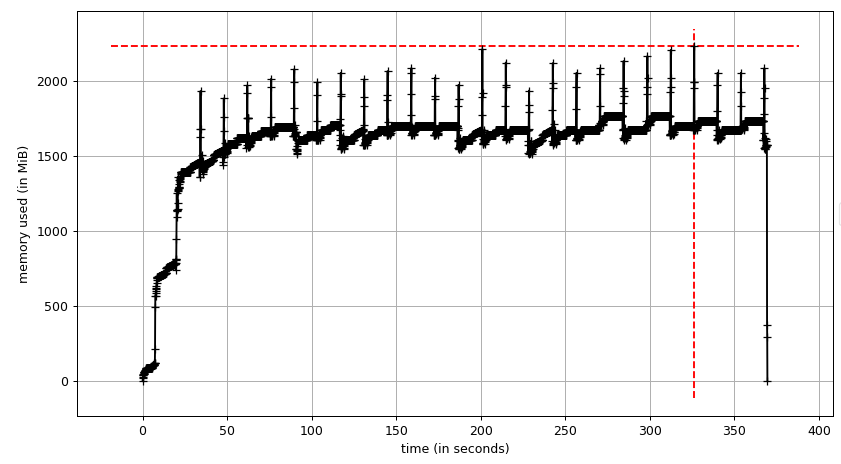
\includegraphics[width=0.5\textwidth]{images/results/sn14_new_bk}}}\hfill
\subfloat[Memoria ocupada en SN18]{\label{fig:new_kbf_18}{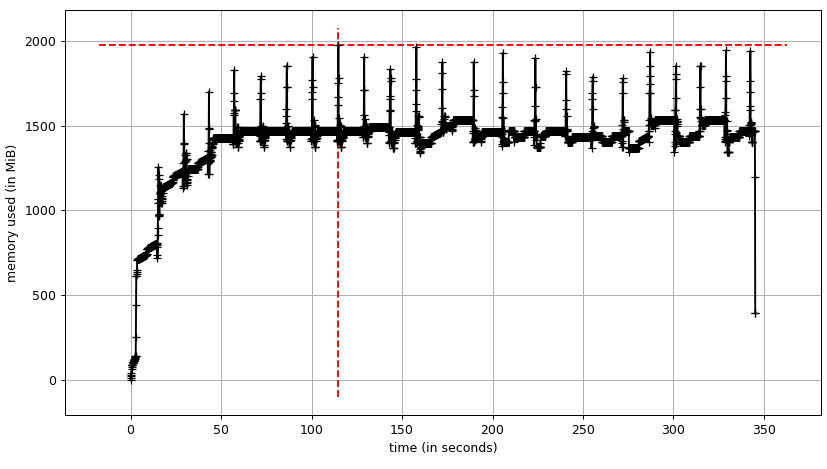
\includegraphics[width=0.5\textwidth]{images/results/sn18_new_bk}}}\vfill
\subfloat[Memoria ocupada en SN80]{\label{fig:new_kbf_80}{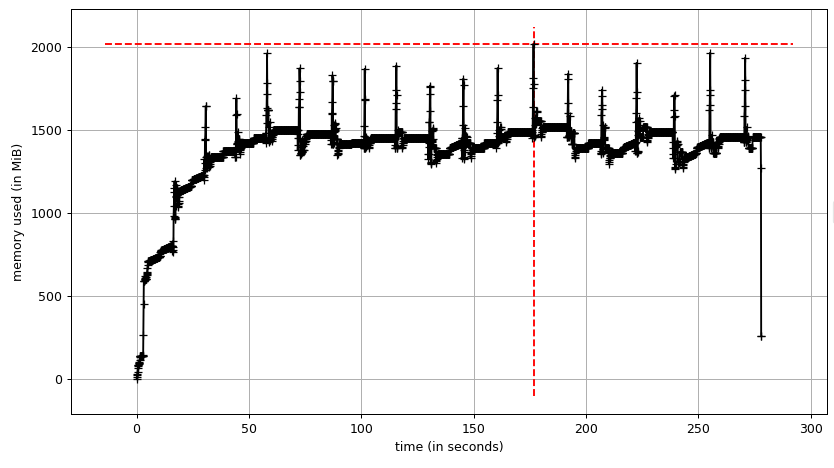
\includegraphics[width=0.5\textwidth]{images/results/sn80_new_bk}}}
\caption{Comportamiento de la memoria (en mebibytes) durante la ejecuci\'on para los tres conjuntos de datos usando el filtro de Kalman B\'asico.}
\label{fig:mem_new_kbf}
\end{figure}

De la Figura \ref{fig:mem_new_kbf} se desprenden los m\'aximos alcanzados durante cada ejecuci\'on con el filtro b\'asico. Los resultados en megabytes se listan en la tabla \ref{tab:mem3}.
\pagebreak

\begin{table}[h!]
\centering
\caption{Memoria principal (en unidades de MB) usada durante la ejecuci\'on del programa refctorizado usando filtro de Kalman B\'asico.}
\begin{tabular}{|l|l|}
\hline
\textbf{ID} & Memoria [MB]\\\hline\hline
SN14 & 2347.78\\\hline
SN18 & 2254.93\\\hline
SN80 & 2365.07\\\hline
\end{tabular}
\label{tab:mem3}
\end{table}


\begin{figure}[h!]
\centering
\subfloat[Memoria ocupada en SN14]{\label{fig:new_mcc_14}{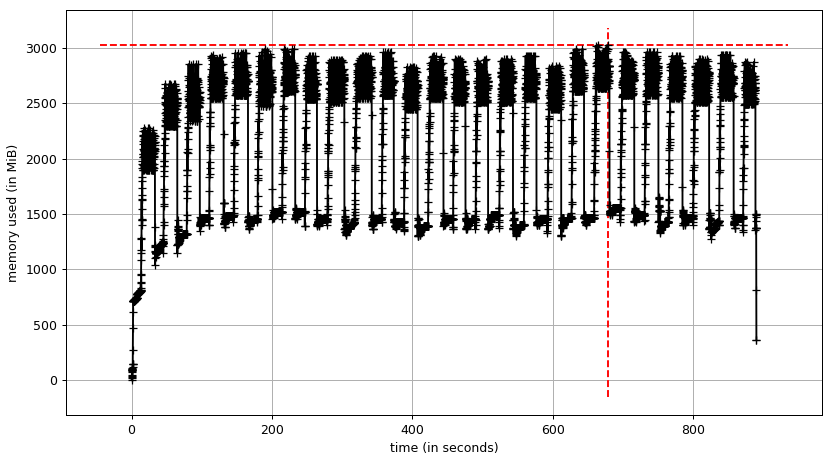
\includegraphics[width=0.5\textwidth]{images/results/sn14_new_mcc}}}\hfill
\subfloat[Memoria ocupada en SN18]{\label{fig:new_mcc_18}{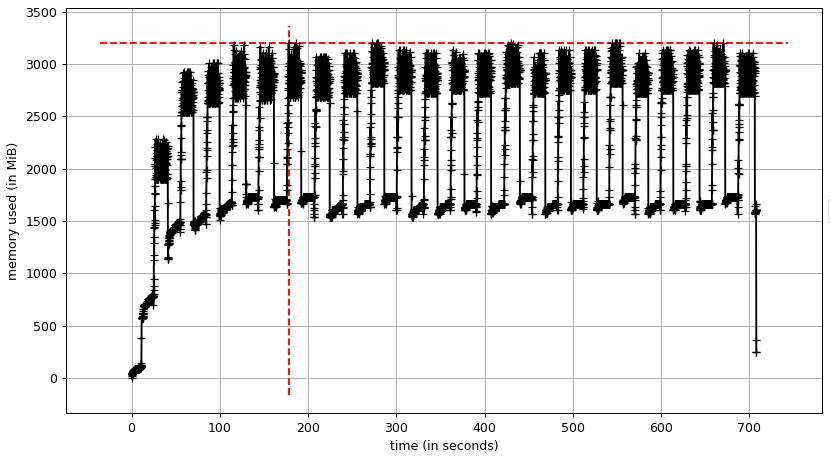
\includegraphics[width=0.5\textwidth]{images/results/sn18_new_mcc}}}\vfill
\subfloat[Memoria ocupada en SN80]{\label{fig:new_mcc_80}{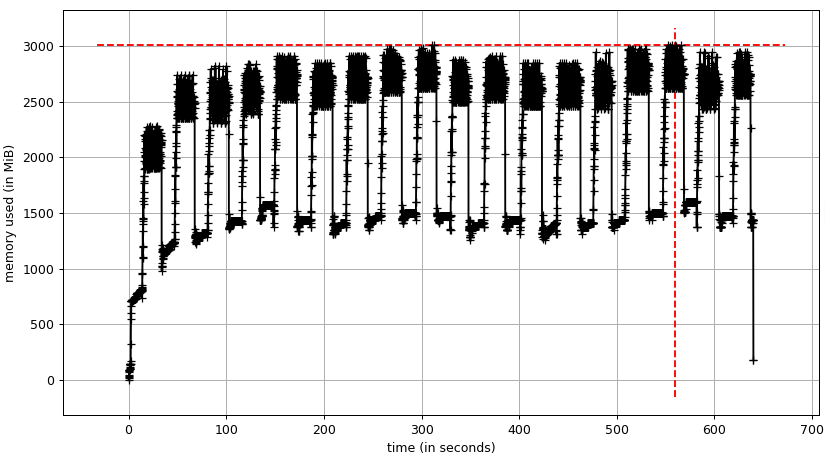
\includegraphics[width=0.5\textwidth]{images/results/sn80_new_mcc}}}
\caption{Comportamiento de la memoria (en mebibytes) durante la ejecuci\'on para los tres conjuntos de datos. En los tres lanzamientos se us\'o el filtro de Kalman de m\'axima correntrop\'ia.}
\label{fig:mem_new_mcc}
\end{figure}

De las series mostradas en la figura \ref{fig:mem_new_mcc} se obtienen los m\'aximos alcanzados de memoria principal ocupada al utilizar el filtro de m\'axima correntrop\'ia listados en la Tabla \ref{tab:mem4}. 
\bigskip

\begin{table}[h!]
\centering
\caption{Memoria principal (en unidades de MB) usada durante la ejecuci\'on del programa refactorizado usando filtro de Kalman de m\'axima correntrop\'ia.}
\begin{tabular}{|l|l|}
\hline
\textbf{ID} & Memoria [MB]\\\hline\hline
SN14 & 3359.54\\\hline
SN18 & 3350.53\\\hline
SN80 & 3330.93\\\hline
\end{tabular}
\label{tab:mem4}
\end{table}

\begin{figure}[h!]
\centering
\subfloat[Memoria ocupada en SN14]{\label{fig:ukf_sn14}{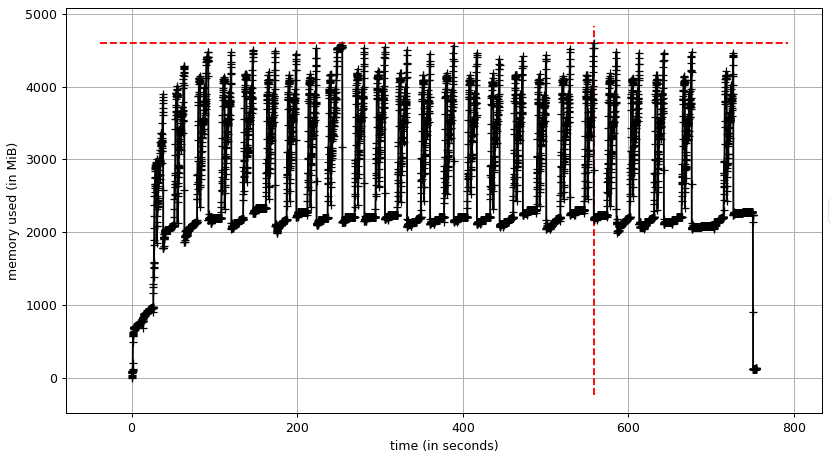
\includegraphics[width=0.5\textwidth]{images/results/sn14_ukf}}}\hfill
\subfloat[Memoria ocupada en SN18]{\label{fig:ukf_sn18}{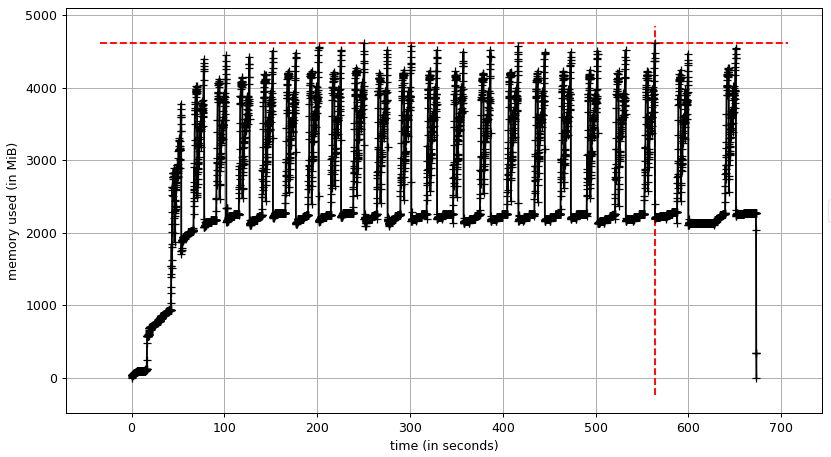
\includegraphics[width=0.5\textwidth]{images/results/sn18_ukf}}}\vfill
\subfloat[Memoria ocupada en SN80]{\label{fig:ukf_sn80}{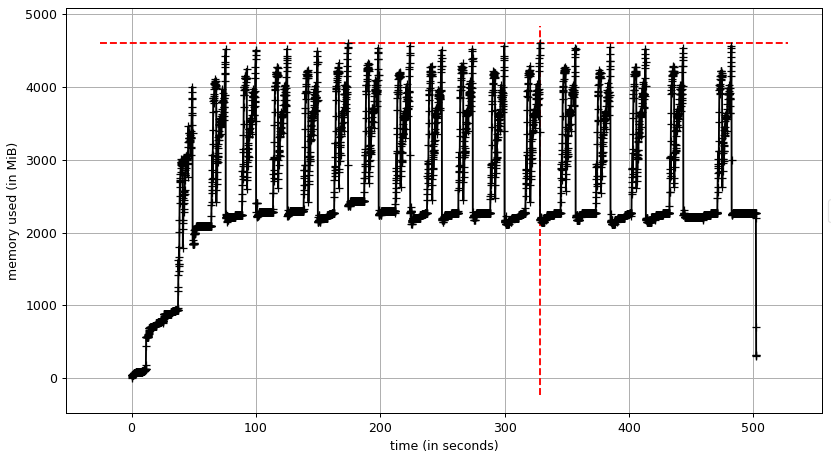
\includegraphics[width=0.5\textwidth]{images/results/sn80_ukf}}}
\caption{Comportamiento de la memoria (en mebibytes) durante la ejecuci\'on para los tres conjuntos de datos. En los tres lanzamientos se us\'o el filtro de Kalman de unscented.}
\label{fig:mem_ukf}
\end{figure}

Los m\'aximos de uso de memoria principal al emplear el filtro unscented, para cada conjunto de datos, se muestra en la Tabla \ref{tab:mem5}.

\begin{table}[h!]
\centering
\caption{Memoria principal (en unidades de MB) usada durante la ejecuci\'on del programa refactorizado usando filtro de Kalman unscented.}
\begin{tabular}{|l|l|}
\hline
\textbf{ID} & Memoria [MB]\\\hline\hline
SN14 & 4827.82\\\hline
SN18 & 4835.96\\\hline
SN80 & 4821.89\\\hline
\end{tabular}
\label{tab:mem5}
\end{table}

Los resultados de memoria principal muestran un uso intensivo de esta al usar el filtro unscented. Esto puede ser debido a la serie de operaciones lineales que se debe realizar al momento de predecir y corregir. Tambi\'en se desprende que el uso de memoria es menor con el filtro b\'asico.
\bigskip
 
\section{Detecci\'on}
%En esta secci\'on se detallan los resultados obtenidos para esta nueva pipeline sobre los datos en las 93 supernovas conocidas. Para todos los filtros listados se emple\'o un threshold de flujo de 200 y de velocidad de flujo de 50.
\subsection{Filtros b\'asico y de m\'axima correntrop\'ia}
La Tabla \ref{tab:tpfn_new} muestra los resultados obtenidos con la nueva versi\'on de la pipeline, empleando los filtros refactorizados de la familia strategy.
\begin{table}[h!]
\centering
\caption{N\'umero de falsos negativos (FN) y verdaderos positivos (TP) encontrados usando cada uno de los filtros. No se observan diferencias entre los resultados de cada filtro refactorizado. La tercera columna de valores muestra la cantidad de conjuntos de datos que no puedieron ser procesados.}
\begin{tabular}{|l|l|l|l|}
\hline
\textbf{Filtro} & \textbf{TP} & \textbf{FN} & \textbf{NaN}\\ \hline
Básico          & 37          & 56          &  3 \\ \hline
MCC             & 37          & 56          & 3 \\ \hline
\end{tabular}
\label{tab:tpfn_new}
\end{table}
\bigskip

Los resultados muestran que para el programa refactorizado tanto el filtro b\'asico como el de correntrop\'ia m\'axima detectan la misma cantidad de supernovas de HiTS. De acuerdo a la informaci\'on dispuesta en la secci\'on \ref{ap:pip_ref} ap\'endice, donde se muestra la tabla \ref{ap:tab2}, se desprende que tampoco hay diferencias de los tiempos o \'epocas de detecci\'on.
\bigskip

Al comparar las tablas \ref{ap:tab1}, correspondiente a los tiempos de detecci\'on en MJD de las implementaciones originales de los filtros y \ref{ap:tab2} a los tiempos de las versiones refactorizadas, se deduce que las detecciones con el \'ultimo grupo de filtros ocurren, cuando es el caso, en la misma \'epoca o antes (horas o d\'ias). Por ejemplo, en las im\'agenes \ref{fig:orig_det_snL} y  \ref{fig:orig_det_snaa} las detecciones se realizan en 57072.145 y 57075.12 con el nuevo conjunto de filtros.
En otras ocasiones, alguno de los grupos no detecta la supernova y en el peor de los casos ninguno de los dos reconoce la supernova.
\bigskip
  

\subsection{Filtro unscented}
Una vez que se pasen las pruebas (\texttt{unittests}) de correctitud, se proceder\'a a ejecutar las pruebas del filtro Unscented en Leftraru.